\documentclass{csse4400}

% \teachermodetrue

\usepackage{languages}

\title{Deploying with Terraform}
\author{Brae Webb}

\date{\week{3}}
\begin{document}

\maketitle

\section{Before Class}
Ensure you've had practice using the AWS Academy learner lab.
It's preferable if you already have \link{terraform installed}{https://learn.hashicorp.com/tutorials/terraform/install-cli}.
Please also have one of IntelliJ IDEA, PyCharm, or VSCode with the terraform plugin installed.

\noindent It is also helpful to have read the Infrastructure as Code lecture notes to understand the motivation for using a tool like Terraform.

\section{This Week}
This week our goal is to get experience using an Infrastructure as Code tool, specifically, Terraform,
to deploy a service to AWS.
Specifically, this week you need to:
\begin{itemize}
    \item Authenticate terraform to use the AWS learner lab.
    \item Configure a single server website in terraform and deploy.
    \item Create a terraform module for deploy arbitrary single server websites.
\end{itemize}

\section{Using Terraform in AWS Leaner Labs}
Following the steps from the week one practical, start a learner lab in AWS Academy.
For this practical, you don't need to create any resources in the AWS Console.
The console can be used to verify that terraform has correctly provisioned resources.

\begin{enumerate}
\item Once the learner lab has started, click on `AWS Details' to display information about the lab.

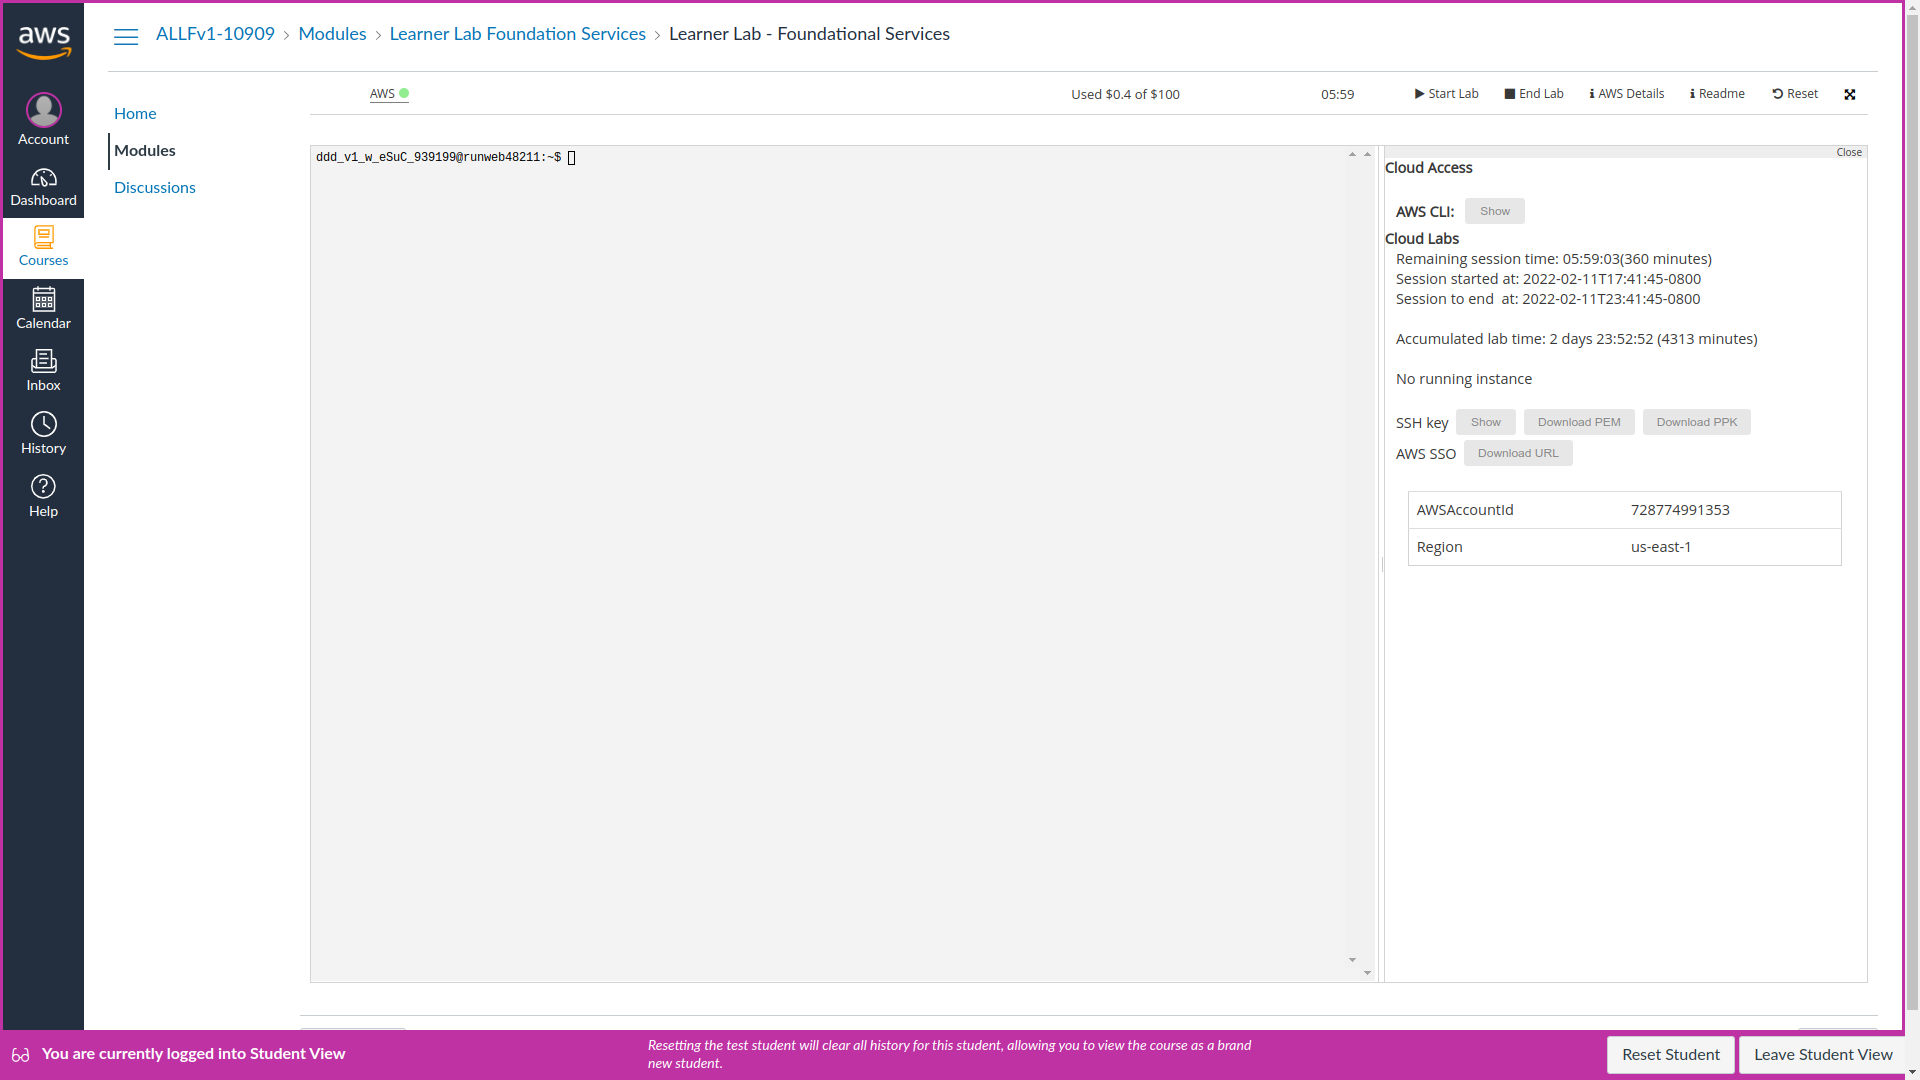
\includegraphics[width=0.7\textwidth]{images/aws-details}

\item Click on the first `Show' button next to `AWS CLI' which will display a text block starting with \texttt{[default]}.
\item Create a directory for this weeks practical.
\item Within that directory create a \texttt{credentials} file and copy the contents of the text block into the file.
\textbf{Don't share this file contents --- don't commit it}.
\item Create a \texttt{main.tf} file in the same directory with the following contents:
\begin{code}[language=terraform]{main.tf}
terraform {
    required_providers {
        aws = {
            source  = "hashicorp/aws"
            version = "~> 3.0"
        }
    }
}

provider "aws" {
    region = "us-east-1"
    shared_credentials_file = "./credentials"
}
\end{code}

The \texttt{terraform} block specifies the required external dependencies, here we need to use the AWS provider.
The \texttt{provider} clock configures the AWS provider, instructing it which region to use and how to authenticate (using the credentials file we created).

\item We need to initialise terraform which will fetch the required dependencies. This is done with the \texttt{terraform init} command.
\bash{terraform init}

This command will create a \texttt{.terraform} directory which stores providers and a provider lock file, \texttt{.terraform.lock.hcl}.

\item To verify that we've setup terraform correctly, use \texttt{terraform plan}.
\bash{terraform plan}

As we currently have no resources configured, it should find that no changes are required.
Note that this doesn't ensure our credentials are correctly configured as terraform has no reason to try authenticating yet.

\end{enumerate}

\section{Deploying Hextris}
If you followed the default instructions in the week one practical, you would have manually deployed the hextris game.
Now we'll try to deploy hextris using terraform.

First, we'll need to create an EC2 instance resource.
The AWS provider calls this resource an \link{\texttt{aws\_instance}}{https://registry.terraform.io/providers/hashicorp/aws/latest/docs/resources/instance}.
Get familiar with the documentation page.
Most terraform providers have reasonable documentation, reading the argument reference section helps to understand what a resource is capable of.

We'll start off with the basic information for the resource.
We configured it to use a specific AMI and chose the \texttt{t2.micro} size.
Refer back to the week one practical sheet for a refresher.
Add the following basic resource to \texttt{main.tf}:

\begin{code}[language=terraform]{main.tf}
resource "aws_instance" "hextris-server" {
    ami           = "ami-0a8b4cd432b1c3063"
    instance_type = "t2.micro"
    
    tags = {
        Name = "hextris"
    }
}      
\end{code}

Let's create this server.
\texttt{terraform apply} will first do \texttt{terraform plan} and prompt us to confirm if we want to apply to changes.

\bash{terraform apply}

You should be prompted with something similar to the output below.

\begin{code}[language=terraform-plan]{}
Terraform used the selected providers to generate the following execution plan. Resource actions are indicated with the following symbols:
  + create

Terraform will perform the following actions:

  # aws_instance.hextris-server will be created
  + resource "aws_instance" "hextris-server" {
      + ami                                  = "ami-0a8b4cd432b1c3063"
      (omitted)
      + instance_type                        = "t2.micro"
      (omitted)
      + tags                                 = {
          + "Name" = "hextris"
        }
    }

Plan: 1 to add, 0 to change, 0 to destroy.

Do you want to perform these actions?
  Terraform will perform the actions described above.
  Only 'yes' will be accepted to approve.

  Enter a value: 
\end{code}

If the plan looks sensible enter \texttt{yes} to enact the changes.

\begin{code}[language=terraform-plan]{}
  Enter a value: yes

aws_instance.hextris-server: Creating...
aws_instance.hextris-server: Still creating... [10s elapsed]
aws_instance.hextris-server: Still creating... [20s elapsed]
aws_instance.hextris-server: Still creating... [30s elapsed]
aws_instance.hextris-server: Still creating... [40s elapsed]
aws_instance.hextris-server: Creation complete after 47s [id=i-08c92a097ae7c5b18]

Apply complete! Resources: 1 added, 0 changed, 0 destroyed.
\end{code}

You can now check in the AWS Console that an EC2 instance with the name \texttt{hextris} has been created.
Now we've got a server, we should try to configure it to contain hextris.
We'll use the \texttt{user\_data} field which configures commands to run when launching the instance.
First we need a script to provision the server, if we combine all our commands from the last practical, we'll produce this script:

\begin{code}[language=bash]{deploy.sh}
#!/bin/bash
yum install -y httpd
systemctl enable httpd
systemctl start httpd

yum install -y git
cd /var/www/html
git clone https://github.com/Hextris/hextris .  
\end{code}

\teacher{The hash bang is required.}

\teacher{Don't forget the -y on yum install}

Now we can add the following field to our terraform resource.
It uses the terraform \texttt{file} function to load the contents of a file named \texttt{deploy.sh} relative to the terraform directory.
The contents of that file is passed to the \texttt{user\_data} field.

\begin{code}[language=terraform]{}
user_data = file("${path.module}/deploy.sh")
\end{code}

If you run the \texttt{terraform plan} command now,
you'll notice that terraform has identified that this change will require creating a new EC2 instance.
Where possible, terraform will try to update a resource in-place but since this changes how an instance is started, it needs to be replaced.
Go ahead and apply the changes.

Now, in theory\footnote{hint}, we should have deployed hextris to an EC2 instance.
But how do we access that instance?
We \textsl{could} go to the AWS Console and find the public IP address.
However, it turns out that terraform already knows the public IP address.
In fact, if you open the terraform state file (\texttt{terraform.tfstate}),
you should be able to find it hidden away in there.
But we don't want to go hunting through this file all the time.
Instead we'll use the \texttt{output} keyword.

We can specify certain attributes as `output' attributes.
Output attributes are printed to the terminal when the module is invoked directly
but as we'll see later, they can also be used by other terraform configuration files.

\begin{code}[language=terraform]{main.tf}
output "hextris-url" {
  value = aws_instance.hextris-server.public_ip
}
\end{code}

This creates a new output attribute, \texttt{hextris-url},
which references the \texttt{public\_ip} attribute of our \texttt{hextris-server} resource.
Note that resources in terraform are addressed by the resource type (\texttt{aws\_instance})
followed by the name of the resource (\texttt{hextris-server}).

If you plan or apply the changes it should tell you the public IP address of the instance resource.
\bash{terraform plan}

\begin{code}[language=terraform-plan]{}
aws_instance.hextris-server: Refreshing state... [id=i-043a61ff86aa272e0]

Changes to Outputs:
  + hextris-url = "3.82.225.65"

You can apply this plan to save these new output values to the Terraform state, without changing any real infrastructure.  
\end{code}

So let's try and access that url, hmm.
That's strange. Something's gone wrong.

\section{Security Groups}
As you'll recall from the practical in week one.
An important part of setting up the EC2 instance was configuring the security group to allow traffic from port 80 to reach the instance.
Configuring the security group was built into the process with the GUI configuration.
When configuring with terraform, security groups and their attachment to EC2 instances are separate resources.
Refer back to the terraform documentation for details or,
as is normally quicker, \href{https://www.google.com/search?q=terraform+aws+security+group}{Google ``terraform aws security group''}.

First, let's create an appropriate security group.
Recall the in the GUI configuration,
ingress SSH access (port 22) and all egress%
\footnote{Ingress and egress in networking just means incoming and outgoing respectively.}
traffic was automatically configured and we just added ingress port 80.
In terraform the whole state must be configured so we specify two
\texttt{ingress} blocks one for HTTP (port 80) and one for SSH access (port 22).%
\footnote{We won't actually need SSH access as all the server configuration is done when the machine is provisioned thanks to the \texttt{user\_data},
but we'll try to recreate the instance from the week one practical exactly.}
Additionally, we'll create egress for all outgoing traffic.

\begin{code}[language=terraform]{}
resource "aws_security_group" "hextris-server" {
  name = "hextris-server"
  description = "Hextris HTTP and SSH access"

  ingress {
    from_port = 80
    to_port = 80
    protocol = "tcp"
    cidr_blocks = ["0.0.0.0/0"]
  }

  ingress {
    from_port = 22
    to_port = 22
    protocol = "tcp"
    cidr_blocks = ["0.0.0.0/0"]
  }

  egress {
    from_port = 0
    to_port = 0
    protocol = "-1"
    cidr_blocks = ["0.0.0.0/0"]
  }
}
\end{code}

Note the following:
\begin{itemize}
  \item \texttt{from\_port} and \texttt{to\_port} are the start and end of a range of ports rather than incoming or outgoing. In this example our range is 80-80.
  \item \texttt{protocol} set to -1 is a special flag to indicate all protocols.
  \item Explaining \texttt{cidr} is outside the scope of the course, but the specified block above means to apply to all IP addresses.
\end{itemize}

You may now apply the changes to create this new security group resource.

Next, we'll attach the security group to the EC2 instance.
Return to the \texttt{aws\_instance.hextrix-server} resource
and include the following line:

\begin{code}[language=terraform]{}
security_groups = [aws_security_group.hextris-server.name]
\end{code}

Note that EC2 instances can have multiple security groups.
Once again notice the structure of resource identifiers in AWS.

% Now if we try to apply or plan these changes,
% we'll noticed that the change of security group forces replacement.
% TODO: I don't actually know why it does this.

Now apply the changes.
If you now try to access via the IP address
(the IP address may have changed),
you should be able to view the hextris website.

\section{Tearing Down}

One of the important features of Infrastructure as Code (IaC) is all the configuration we just did is stored in a file.
This file can, and should be, version controlled and subject to the same quality rules of code files.
It also means that if we want to redeploy Hextris at any point,
we can easily just run the IaC to deploy it.

To try this out, let's first take everything down.
We can do this with:
\bash{terraform destroy}

You should be prompted to confirm that you want to destroy all of the resources in the state.
Once terraform has finished taking everything down,
confirm that you can no longer access the website and that the AWS console says the instances have been destroyed.

Now go ahead and do apply the changes to bring everything back:
\bash{terraform apply}

Confirm that this brings the website back exactly as before (with a different IP address).
You can now start any lab you want and almost instantly spin back up the website you've configured.
That's the beauty of Infrastructure as Code!

Hint: destroy everything again before you leave.

\bibliographystyle{ieeetr}
\bibliography{references}

\appendix

% \teacher{
\section{AWS Networking Terminology}
\paragraph{AWS Regions}
Regions are the physical locations of AWS data centres.
When applying terraform, the changes are being made to one region at a time.
In our case we specified the region \texttt{us-east-1}.
Often you don't need to deploy to more than one region, however,
it can help decrease latency and reduce risk from a major disaster.
Generally, pick a region and stick with it,
we've picked \texttt{us-east-1} because it's the least expensive.

\begin{figure}[ht]
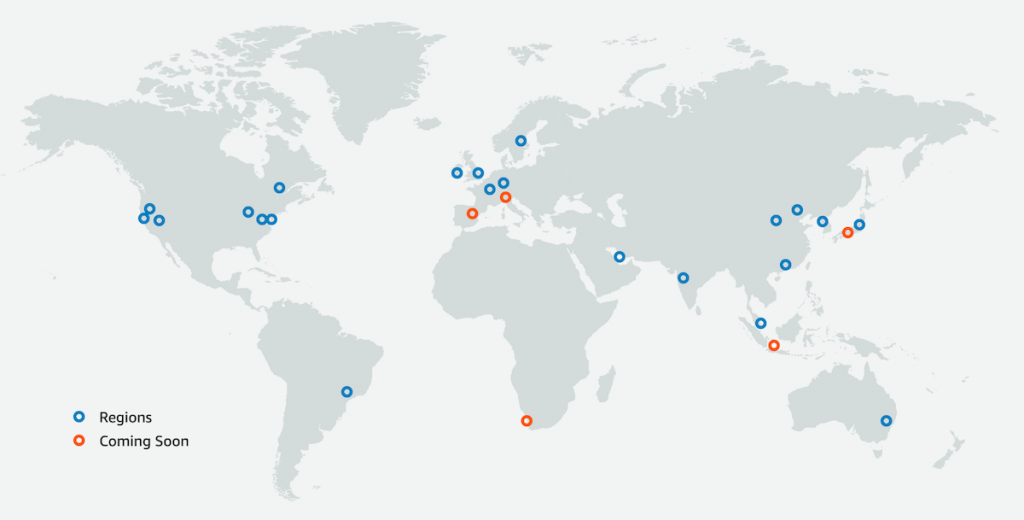
\includegraphics[width=\textwidth]{images/aws_regions}
\caption{AWS Regions as of March 2020 \cite{aws-regions}}
\end{figure}

\paragraph{Availability Zones}
An AWS Region will consist of availability zones, normally named with letters.
For example, the AWS Region located in Sydney, \texttt{ap-southeast-2} has three availability zones:
\texttt{ap-southeast-2a}, \texttt{ap-southeast-2b}, and \texttt{ap-southeast-2c}.
An availability zone is a collection of resources which run on separate power supplies and networks.
Essentially minimising the risk that multiple availability zones would fail at once.

\paragraph{VPC}
Virtual Private Clouds, or VPCs,
are virtual networks under your control,
if you've managed a regular network before it should be familiar.
VPCs are contained within one region but are spread across multiple availability zones.


\end{document}